\documentclass{beamer}
\usepackage[utf8]{inputenc} 
\setbeamerfont{block title}{size={}}
\usepackage[T1]{fontenc}
\usepackage{lmodern}
\usepackage{pifont}
\usepackage{graphicx}
\usepackage[french]{babel}
\usetheme{PaloAlto}
\title[SWU]{SmallWorldUtbm}
\author[]{Amani YOUNES - Gabriel NOTONG - Michael LONGO - Pierre ROGNON}
\institute{Programmation orientée objet - LO43}
\date{11 janvier 2013}
\addtobeamertemplate{footline}{~\hspace*{12cm}\insertframenumber/\inserttotalframenumber}


\usepackage[absolute,showboxes,overlay]{textpos}     % déclaration du package
\textblockorigin{0px}{0px}                               % origine des positions
\TPshowboxesfalse  
 % n'affiche pas le contour des textblock
\usepackage{multimedia} 

\AtBeginSection[]
{
  \begin{frame}<beamer>
    \frametitle{Sommaire}
{\scriptsize\tableofcontents[currentsection]
}
  \end{frame}
}

\begin{document}
\definecolor{bleu}{HTML}{0000B0}
\definecolor{rouge}{HTML}{FF0000}
\definecolor{vert}{HTML}{00B81E}



\begin{frame}
\titlepage
\end{frame}

\section*{Introduction}

\begin{frame}{Introduction}
	
	\begin{itemize}
		\item but du projet: réalisation d'un jeu: SmallWorldUtbm;
		\vspace*{0.3cm}
		\item adaptation du jeu de plateau SmallWorld;
		\vspace*{0.3cm}
		\item projet réalisé en Java, conception faite en UML;
		\vspace*{0.3cm}
	\end{itemize}
	
	\begin{center}
		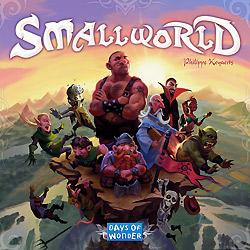
\includegraphics[width=3cm]{smallworld.jpg}
	\end{center}
\end{frame}

\section{Étude du sujet et adaptation}

\begin{frame}{Étude du sujet et adaptation}

	\begin{itemize}
		\item étude basée sur le manuel de règles du jeu;
		\vspace*{0.5cm}
		\item plusieurs concepts adaptés au contexte de l'UTBM:
		\begin{itemize}
			\item les peuples;
			\item les pouvoirs;
			\item les éléments;
			\item la carte.
		\end{itemize}
	\end{itemize}

\end{frame}

	\subsection{Les peuples}

\begin{frame}{Les peuples utbohémiens}

\begin{center}
	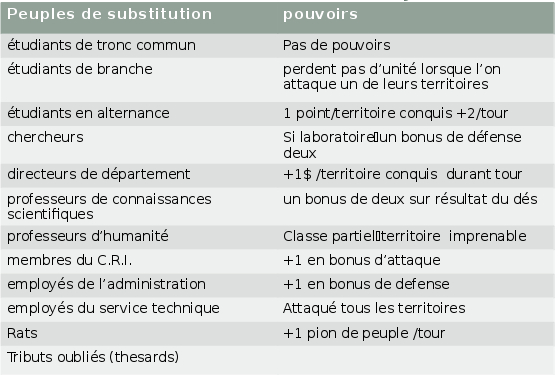
\includegraphics[width=8cm]{peuples.png}
\end{center}

\end{frame}


	\subsection{Les pouvoirs}

\begin{frame}{Les pouvoirs utbohémiens}

\begin{center}
	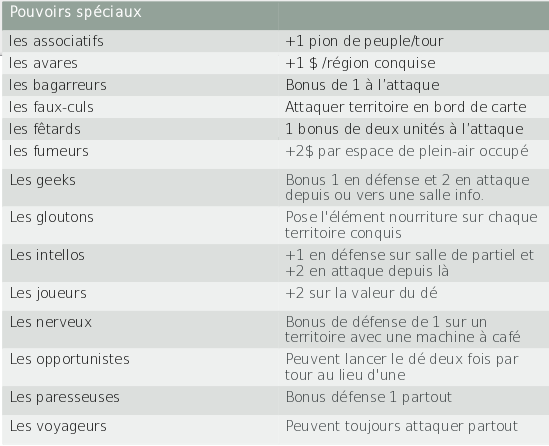
\includegraphics[width=8cm]{pouvoirs.png}
\end{center}

\end{frame}

	\subsection{Les éléments}

\begin{frame}{Les éléments utbohémiens}

\begin{center}
	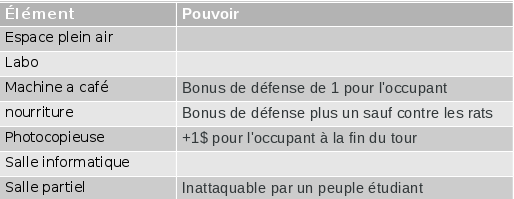
\includegraphics[width=9cm]{elements.png}
\end{center}

\end{frame}

	\subsection{Carte}

\begin{frame}{Carte}

\begin{itemize}
	\item Inspirée des bâtiments de Belfort.
\end{itemize} 

\begin{center}
	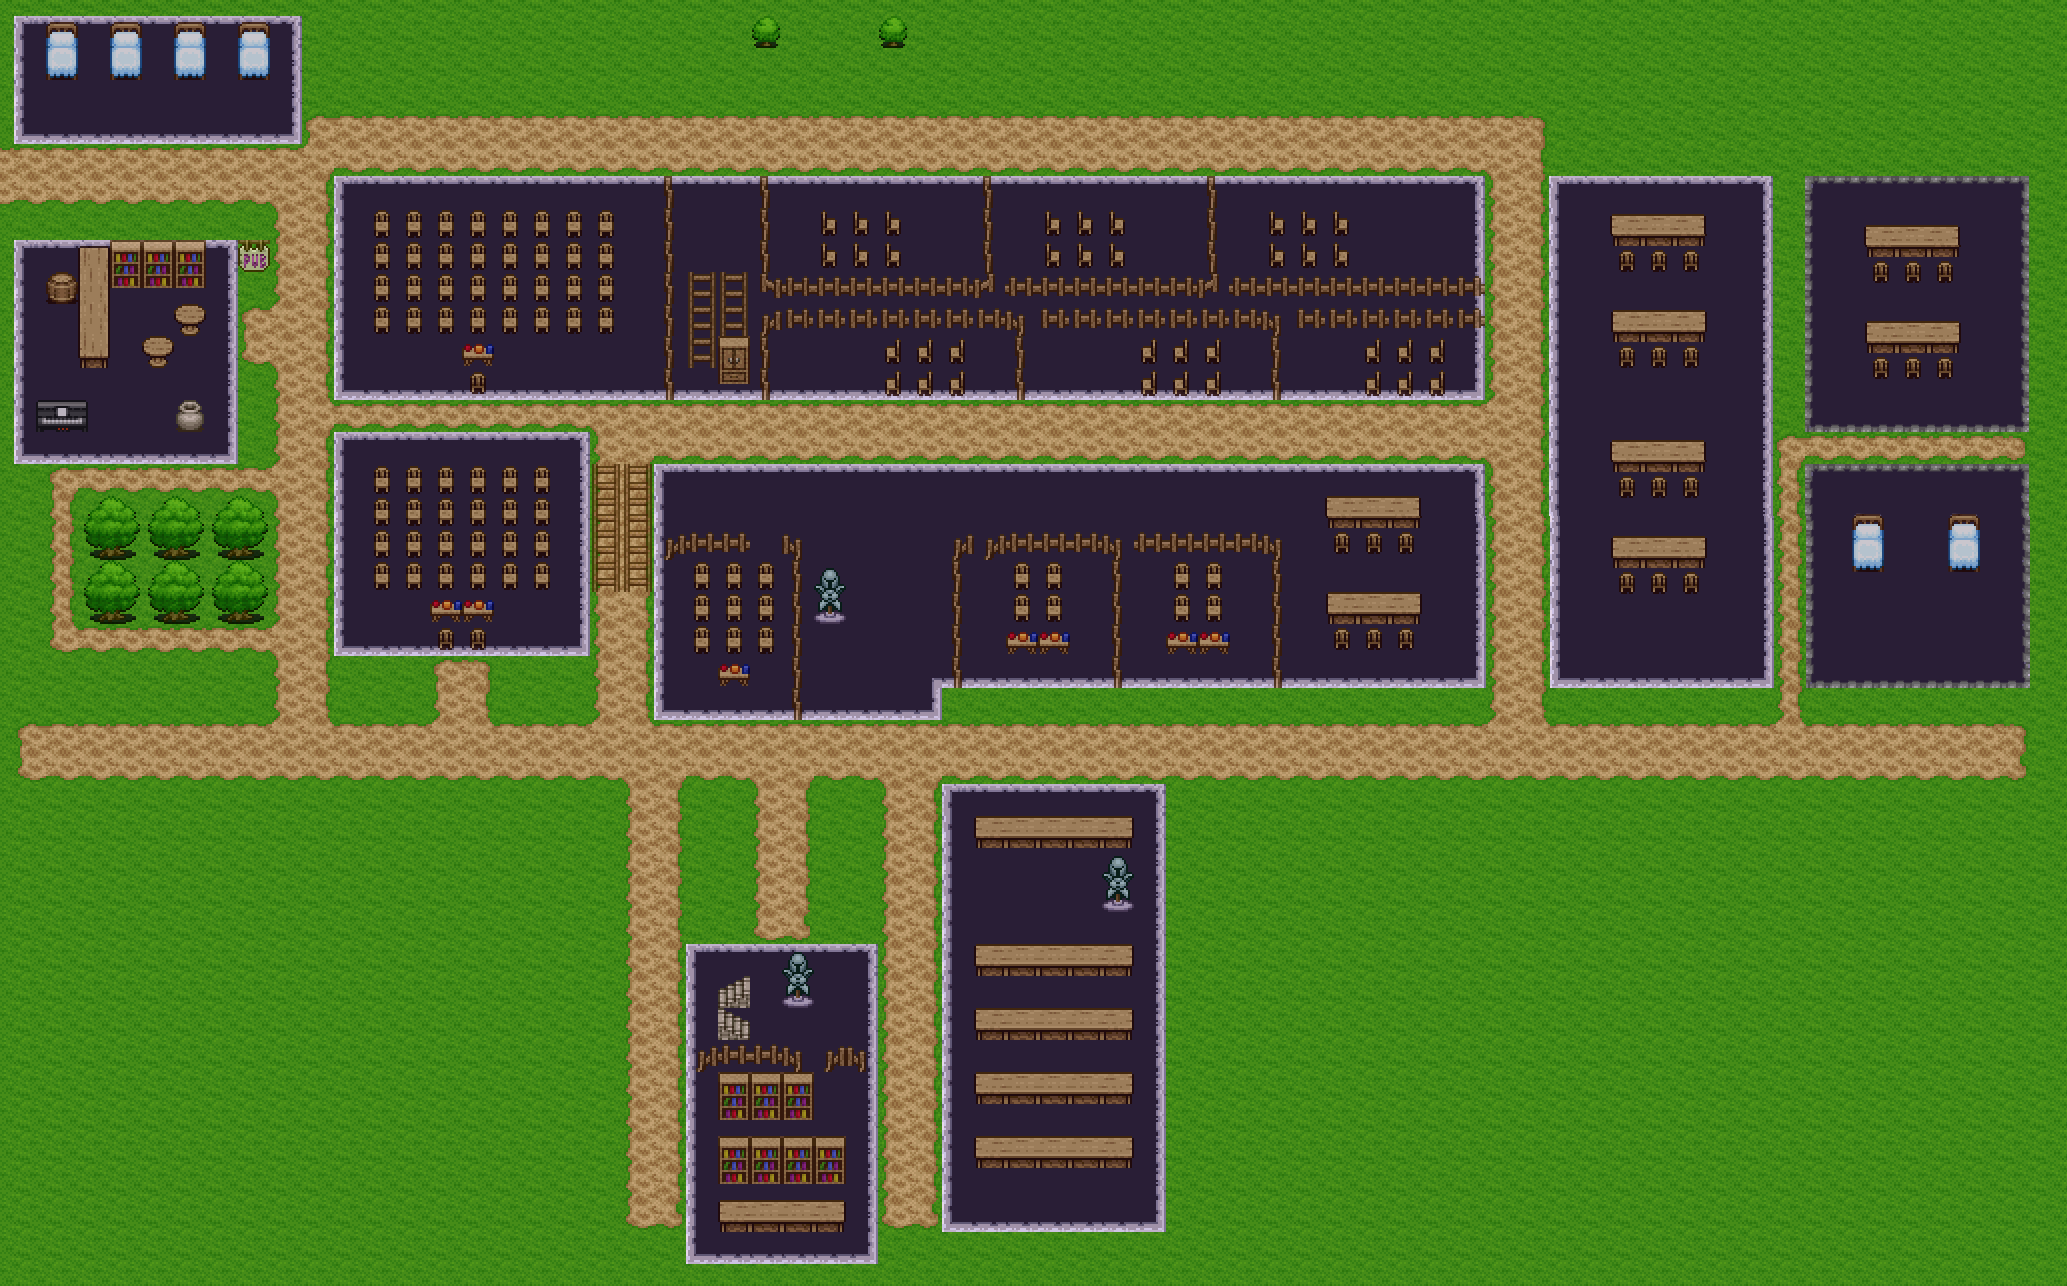
\includegraphics[width=8cm]{mapBelfort.png}
\end{center}

\end{frame}

	\section{Conception}
	
\begin{frame}{Conception}

	\begin{itemize}
		\item réalisation d'un cas d'utilisation;
		\vspace*{0.2cm}
		\item réalisation d'un diagramme de classes;
		\vspace*{0.2cm}
		\item réalisation de quatre diagrammes de séquences.
	\end{itemize}
	\begin{center}
		\vspace*{0.5cm}
		
\includegraphics[width=3cm]{uml.jpg}
	\end{center}
\end{frame}

	\subsection{Cas d'utilisation}
	
\begin{frame}{Cas d'utilisation}

\begin{center}
	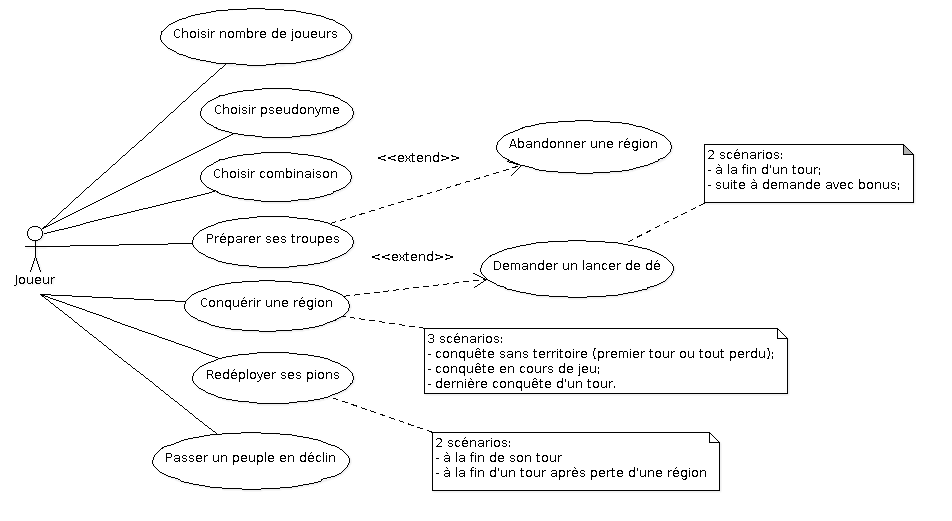
\includegraphics[width=9cm]{DiagrammeDeCasDUtilisation.png}
\end{center}

\end{frame}

	\subsection{Diagramme de classe}
	
\begin{frame}{Diagramme de classes: classe Partie}

	\begin{center}
		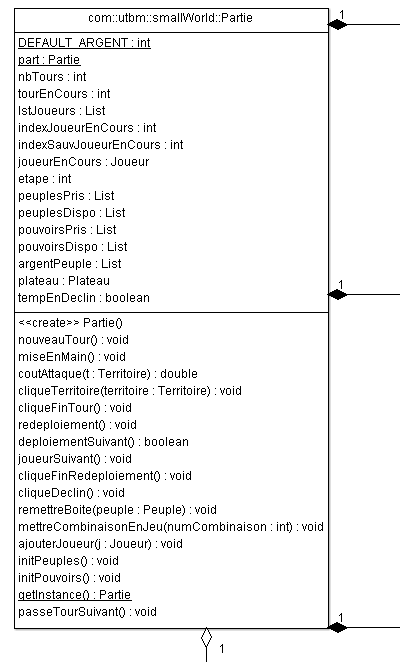
\includegraphics[width=4cm]{partie.png}
	\end{center}

\end{frame}

\begin{frame}{Diagramme de classes: côté joueur}

	\begin{center}
		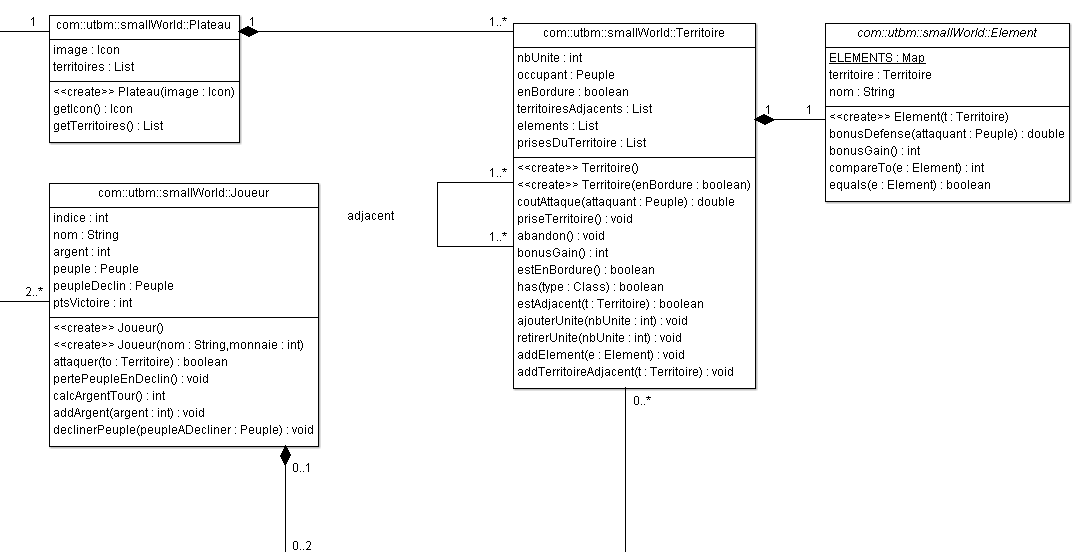
\includegraphics[width=10cm]{cotejoueur.png}
	\end{center}

\end{frame}

\begin{frame}{Diagramme de classes: côté peuple}

	\begin{center}
		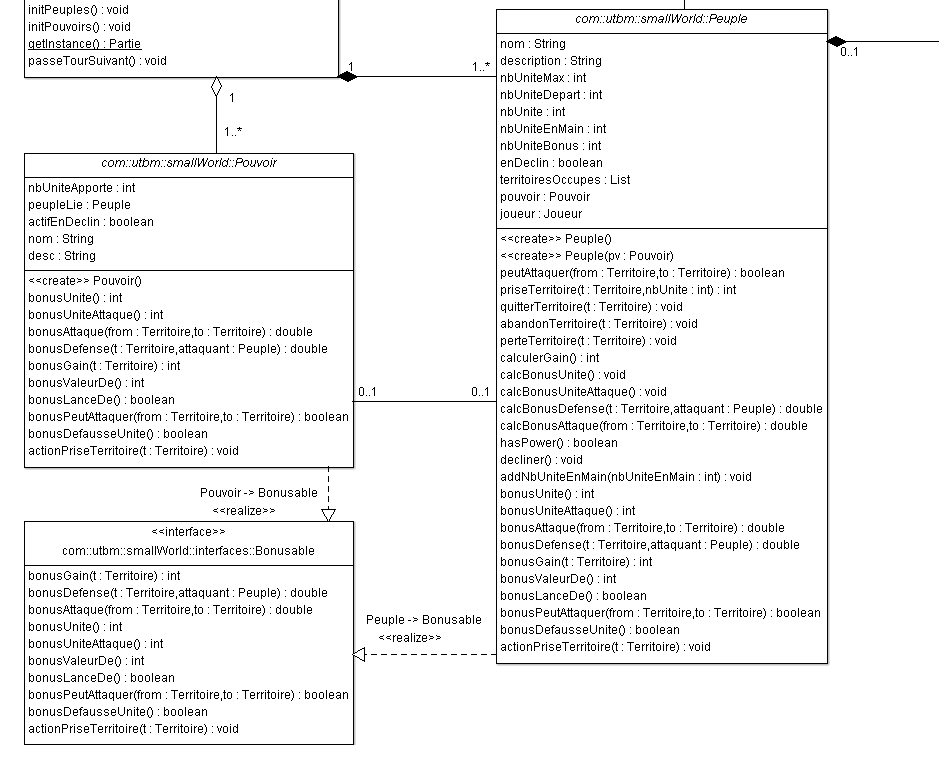
\includegraphics[width=9cm]{cotepeuple.png}
	\end{center}


\end{frame}

	\subsection{Diagramme de séquences}

\begin{frame}{Diagramme de séquences}

\begin{center}
	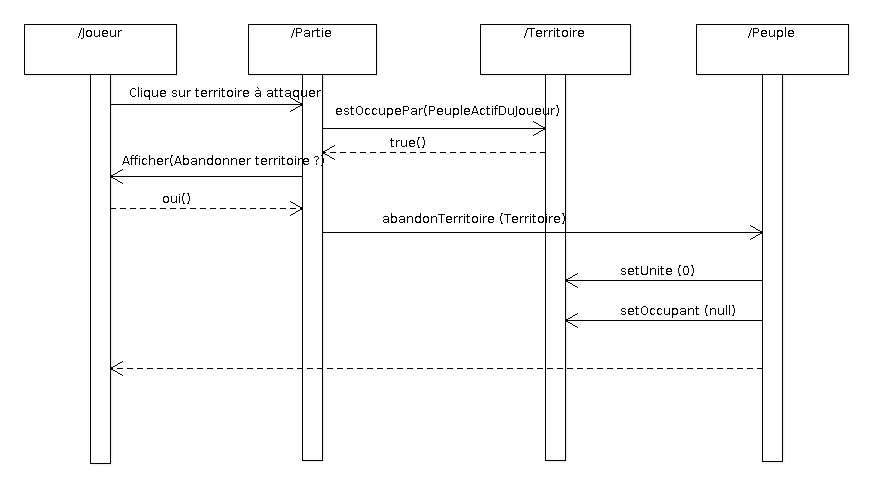
\includegraphics[width=10cm]{DSSAbandon.png}
\end{center}

\end{frame}

	\section{Réalisation}
	
		\subsection{Architecture de l'application}
		
	
\begin{frame}{Architecture de l'application}

	\begin{itemize}
		\item Un package général et un pour chaque "famille" de sous-classes;
		\vspace*{0.2cm}
		\item com.utbm.SmallWorld contient les classes principales;
		\vspace*{0.2cm}
		\item com.utbm.SmallWorld.elements, com.utbm.SmallWorld.peuples, com.utbm.SmallWorld.pouvoirs;					\vspace*{0.2cm}
		\item com.utbm.SmallWorld.interfaces contient Bonusable;
		\vspace*{0.2cm}
		\item com.utbm.SmallWorld.gui les classes graphiques.
	\end{itemize}

\end{frame}

	\subsection{Développement de l'interface}
	
\begin{frame}{Développement de l'interface}

	\begin{itemize}
		\item une classe principale: Game;
		\item des classes implémentant des Listener: JoueurAction, TerritoireCase, Prompt, WinWait;
		\item une classe de connexion à la bdd: SQLite;
		\item des classes implémentant des fenêtres: WinWarn et WinMenu.
	\end{itemize}
	
	\begin{center}
		
\includegraphics[width=3cm]{winwait.png} \hspace*{0.2cm}
		
\includegraphics[width=3.4cm]{winmenu.png}\\
		\vspace*{0.2cm}
		
\includegraphics[width=6.7cm]{winwarn.png}
		
	\end{center}

\end{frame}

	\subsection{Outils utilisés}

\begin{frame}{Outils utilisés}

	\begin{itemize}
		\item le gestionnaire de version git;
		\item l'I.D.E. Eclipse;
		\item Google Doc;
		\item une base de données SQLite;
	\end{itemize}
	
	\begin{center}
		
\includegraphics[width=3cm]{waldocat.jpg} \hspace*{0.5cm}
		
\includegraphics[width=3cm]{eclipse.png}
	\end{center}

\end{frame}

\section{Bilan}

\begin{frame}{Bilan}

	\begin{itemize}
		\item au niveau humain,
		\begin{itemize}
			\item travail en équipe;
			\item découverte de nouvelles personnes;
			\item utilisation de git pour répartir le travail.
		\end{itemize}		
		\vspace*{0.5cm}
		\item au niveau pédagogique:
		\begin{itemize}
			\item pratique de Swing;
			\item utilisation des interfaces;
			\item découverte d'une connexion à une bdd depuis Java.
		\end{itemize}
	\end{itemize}

\end{frame}

\section*{Conclusion}

\begin{frame}{Conclusion}

	\begin{itemize}
		\item un travail terminé et fonctionnel;
		\vspace*{0.5cm}
		\item une conception UML longue mais qui a permis de gagner du temps sur le développement;
		\vspace*{0.5cm}	
		\item un travail enrichissant pour chacun de nous.
	\end{itemize}

\end{frame}


\end{document}


